\documentclass{scrartcl}

\usepackage{multirow}
\usepackage[version=4]{mhchem}

\usepackage{siunitx}
\DeclareSIUnit{\atm}{atm}


\usepackage{longtable}

\usepackage{csvsimple}

\usepackage{booktabs}

\usepackage{graphicx}

\usepackage{rotating}

\usepackage{caption}

\begin{document}

\section{General}
The nutrients relevant for plant growth are the following:\\\\
\textbf{Macronutrients}
\begin{itemize}
	\item{N}
	\item{P}
	\item{K}
	\item{Ca}
	\item{Mg}
	\item{S}
\end{itemize}
\textbf{Micronutrients}
\begin{itemize}
	\item{Fe}
	\item{Cu}
	\item{Zn}
	\item{B}
	\item{Mn}
	\item{Mo}
	\item{Ni} 
\end{itemize}
The solubility of a salt is generally determined by 
\begin{itemize}
	\item{its solubility product ($K_{S0}$),}
	\item{the temperature ($\text{T}$),}
	\item{the pH, affecting speciation,}
	\item{the pE, affecting speciation,}
	\item{the partial pressure of \ce{CO2}(g) ($p_{\ce{CO2}}$,}
	\item{the presence of common ions,}
	\item{the ionic strength of the solution,}
	\item{and the presence of chelating agents.}
\end{itemize}
%
The solids with the lowest solubility are assumed to control the total solubility of the contained compounds in aquatic systems.\\
The \textbf{pH} of an aquaculture system would typically range between \SIrange{6.5}{8.0}. A higher pH would lead to an equilibrium shift of the chemical equilibrium between \ce{NH4+} and \ce{NH3}
\begin{align}
	\ce{NH4+ + OH- <=> NH3 + H2O}	
\end{align}
, with \ce{NH3} being a toxic species for fish. It is thus not desirable to raise the pH above a value of 8. On the other hand, a low pH leads to the shift of the equilibrium between \ce{NO3-} and \ce{HNO3}
\begin{align}
	\ce{NO3- + H3O+ <=> HNO3 + H2O}
\end{align}
, with the latter being a toxic component. Furthermore, the decreased pH hampers the transport of \ce{CO2} into the adjacent water and thus poses direct physiological implications for the fish. A third downside of a low pH is the decrease of nitrification efficiency due to suboptimum conditions for nitrifying bacteria.\\
%
The average \textbf{temperature} depends on the fish species reared, while the temperature range is determined by whether the system is cooled or heated using technical equipment or exposed to natural fluctuations. In most aquaponic systems, the species of choice are either African catfish (\emph{Clarias gariepinus}) or Nile tilapia (\emph{Oreochromis niloticus}) with an average temperature preference of \SI{25}{\degreeCelsius}. The fish production system in aquaponics would usually be a recirculation aquaculture system (RAS) with temperature control. Fluctuations are thus expected to be within a range of \SI{1}{\degreeCelsius}. 
%
%
%
\subsection{Hydroxides}
The formation of hydroxides is determined by the pH. With increasing pH, the concentration of \ce{OH-} ions increases as well.
%
%
%
\subsection{Carbonates}
Aquaculture systems can be considered open systems where the partial pressure of \ce{CO2}(g) is constant. The total concentration of [\ce{CO2}(aq)] and consequently [\ce{H2CO3}*] is thus depending on the pH and $T$ of the system. Under the conditions in an aquaponic system, and considering $pKa_{2} = 10.4$ of the carbonate system, the availability of free [\ce{CO3^2-}(aq)] is limited. However, carbonate speciation is pH dependent, as visible in Figure \ref{fig:carbonate}. If [\ce{H2CO3}*] is removed due to an increasing pH and shift of the equilibrium towards a higher proportion of [\ce{HCO3-}] and eventually [\ce{CO3^{2-}}], further gaseous \ce{CO2} can be dissolved in water and is thus raising the total concentration of these carbonaceous compounds in the water.
%
\begin{figure}
	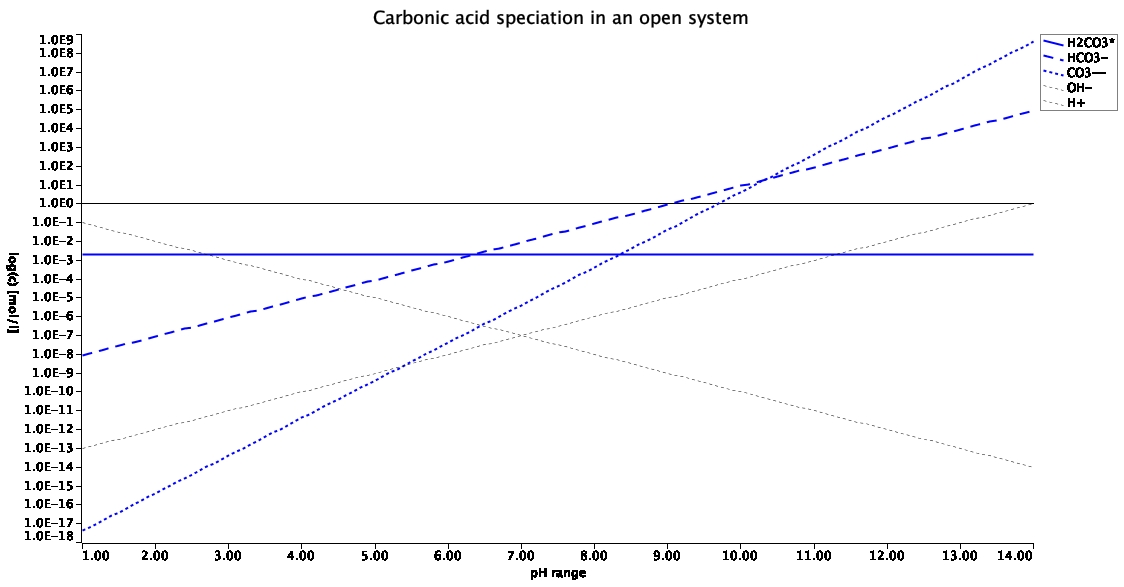
\includegraphics[scale=0.35]{plots/log_carbonic_acid.jpg}
	\caption{Carbonate speciation in an open system}
	\label{fig:carbonate}
\end{figure}
%
%
%
\subsection{Phosphates}
Phosphorus is entering an aquaculture system via the feed. While the average digestibility of phosphorus is ranging between \SIrange{50}{90}{\percent}, the excreted form of phosphorus depends on the form in which it is present in the feed. Phosphorus can be added to the feed in form of phosphate salts, for instance Mono-calcium phosphate, or bound as phytic acid, which is present in plant ingredients and considered as anti-nutritional factor due to its indigestibility. Phosphates are prone to be excreted via the urinary system in form of free ions. Indigestible compounds, on the other hand, are excreted as part of the faeces and are thus considered solids and bound to organic carbon.\\
Phosphate speciation is ph-dependent as can be seen in Figure \ref{fig:phosphate}.
%
\begin{figure}
	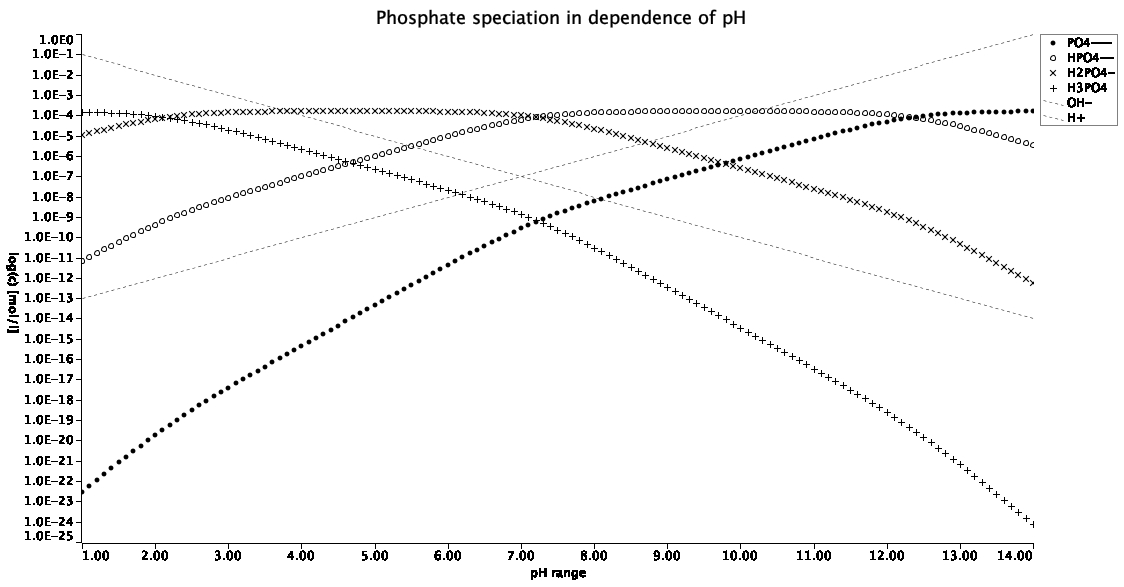
\includegraphics[scale=0.35]{plots/log_phosphates.jpg}
	\caption{Phosphate speciation}
	\label{fig:phosphate}
\end{figure}
%
%
%
\subsection{Nitrates}
%
%
%
\subsection{Sulphates}
As described for phosphates, the speciation of sulphates is heavily depending on the pH of the solution.
%
%
%
\section{Equations and data used}
The dissolution of a salt in \ce{H2O} can be described as
%
\begin{align}
	\ce{A_{m}B_{n} + n H2O <=> m A^{n+} + n B^{m-}}	
	\label{eq:dissolution}
\end{align}
%
. Considering the concentration of \ce{H2O} being constant ($[\ce{H2O}] = 1$), the solubility product $K_{S0}$, which is equal to the ion product of a saturated solution of the salt, can be written as
%
\begin{align}
	K_{S0} = [\ce{A^{n+}}]^{m} \cdot [\ce{B^{m-}}]^{n}
\end{align}
%
in a generalised way. To calculate the maximum solubility $S$ of a salt in \ce{H2O} based on $K_{S0})$, the proportions in which the cation and anion are present in the salt have to be considered as shown in equation \ref{eq:dissolution}. Substitution of the concentration of one ion by the concentration of the other leads to the generalised formula
%
\begin{align}
	S = \sqrt[m+n]{\frac{K_{S0}}{n^{n} \cdot m^{m}}}
\end{align}
%
. The result has then to be multiplied by the corresponding stoichiometric factor resulting from the mass balance of the compounds of the salt.\\
The solubility products used for the calculation of theoretical maximum solubilities of pure salts are given in Table \ref{tab:solubilityProducts}. 
As result of the stoichiometry of the salts
%
%
%
%	TABLE - SOLUBILITY PRODUCTS
%
\begin{table}[!h]
	\caption{Solubility products ($K_{S0}$) of poorly soluble salts of relevant plant nutrients at \SI{25}{\degreeCelsius}.}
	\label{tab:solubilityProducts}
\vspace{5mm}
%
\csvreader[
	before reading	= \begin{center},
	tabular 		= lr,
	table head		= \toprule Compound & Solubility product\\\midrule,
	table foot 		= \bottomrule,
	after reading	= \end{center}
]{Solubility_products.csv}
{Compound = \compound, Solubility product = \constant}{%
\compound & \tablenum{\constant}
}%
\end{table}
%
%
%
\section{Results of calculations}
Initially, the solubilities of the main plant nutrients were calculated using reported mass percentages of a number of their salts at satiation concentration. In case of slightly soluble salts, the satiation concentration was calculated using the solubility product $K_{S0}$.\\
%
%\begin{minipage}{\textwidth}
	\captionof{table}{Calculated solubilities in \si{\mol\per\liter} for a number of salts.}
	\label{tab:solubilityResults}
%
\csvreader[
	before reading	= \begin{center},
	longtable		= lrrr,
	table head 		= \toprule Formula & Salt & Cation & Anion\\\midrule,
	table foot		= \bottomrule,
	after reading	= \end{center}
]{Solubility_calculated.csv}{%
chemFormula = \formula, 
solSaltmol = \salt, 
solCationmol = \cation, 
solAnionmol = \anion
}{%
\formula & \tablenum{\salt} & \tablenum{\cation} & \tablenum{\anion}
}%
%\end{minipage}
%
%
%
The obtained molar concentrations were then converted into mass concentrations.\\
%
%
%
%\begin{minipage}{\textwidth}
%
	\captionof{table}{Calculated solubilities in \si{\milli\gram\per\liter} for a number of salts.}
	\label{tab:solubilityResults}
%
\csvreader[
	before reading	= \begin{center},
	longtable		= llrrr,
	table head 		= \toprule Compound & Formula & Salt & Cation & Anion\\\midrule,
	table foot		= \bottomrule,
	after reading	= \end{center}
]{Solubility_calculated.csv}{%
compound = \compound,
chemFormula = \formula, 
solSaltmg = \salt, 
solCationmg = \cation, 
solAnionmg = \anion
}{%
\compound & \formula & \tablenum{\salt} & \tablenum{\cation} & \tablenum{\anion}
}%
%\end{minipage}




For the following calculations, it is assumed that $\text{pH} = 7.5$, $\text{T} = \SI{25}{\degreeCelsius}$, $\text{K}_{H, \ce{CO2}} = \SI{3.4e-2}{\mol\per\liter\per\atm}$, and $p_{\ce{CO2}} = \SI{5.4e-2}{\atm}$.
%
%
%
\subsection{Hydroxides}
In an aquaculture system with an assumed average pH = 7.5, the hydroxide concentration would be
%
\begin{align}
	[\ce{OH-}] = 10^{-\text{pOH}} = 10^{-(14-\text{pH})} = 10^{-(14-7.5)} = \num{3.2e-7}
\end{align}
.
%
%
%
\subsection{Carbonates}
Assuming that $\text{K}_{H, \ce{CO2}} = \SI{3.4e-2}{\mol\per\liter\per\atm}$, and $p_{\ce{CO2}} = \SI{5.4e-2}{\atm}$, the resulting [\ce{H2CO3^{*}}] would equal to $\approx \SI{2e-3}{\mol\per\liter}$. Within a pH-range from 7 to 8.5, the predominant species would be \ce{HCO3-}, while the concentration of \ce{CO3^{2-}} would range between \SI{4.2e-6}{\mol\per\liter} and \SI{4.2e-3}{\mol\per\liter}.
% 
%
%
\subsection{Phosphates}
The initial mass fraction of all phosphates present in the system was assumed to be \SI{5}{\milli\gram\per\liter}, resulting in a $c_{T}$  of \SI{1.6e-4}{\mol\per\liter}. This data is taken from \cite{Shaw2022}.\\
At a pH = 7, the predominant phosphate species are \ce{H2PO4-} and \ce{HPO4^2-}. Given $c_{T}$, this would result in $[\ce{H2PO4-}] \approx \SI{6e-2}{\mol\per\liter}$ and $[\ce{HPO4^2-}] \approx \SI{4e-2}{\mol\per\liter}$.
%
%
%
\section{Comparison with empirical results}
In the following, theoretical concentrations of compounds relevant for plant nutrition and concentrations found empirically are compared in Table \ref{tab:empirical}. The theoretical concentrations are referring to the maximum concentration possible, considering only solubility product constants and neglecting complexing agents such as humic substances present in the water.
%
%
%
%
%	
\begin{table}[!h]
	\caption{Table}
	\label{tab:empirical}
\vspace{5mm}
%
\end{table}
%
%
%
\section{Discussion}



\end{document}